\documentclass[aspectratio=169,xcolor={usenames,dvipsnames,svgnames,table},10pt,usepdftitle=false,hyperref={bookmarksdepth=3}]{beamer}

\usetheme[titleformat frame=smallcaps, numbering=fraction]{metropolis}
\usefonttheme{professionalfonts}
%\setbeamertemplate{frame footer}{\insertshorttitle\quad---\quad\insertshortauthor}

\usepackage{polyglossia}
\setmainlanguage{german}
\setotherlanguage{english}

\usepackage{appendixnumberbeamer} % Don't count appendix, references etc. in slide count
\usepackage{amsmath,amssymb,amsfonts}
\usepackage{graphicx}
\usepackage{perpage}
\usepackage{enumitem}
\usepackage[absolute,overlay]{textpos}
\usepackage{multirow, booktabs, tablefootnote, wrapfig}

\usepackage{booktabs} % for toprule
\usepackage{tabularx} % alternative tabular environment
\newcolumntype{R}{>{\raggedleft\arraybackslash}X} % custom tabular option

\MakePerPage{footnote}
%\usepackage{graphicscache} % automatic image size reduction (comment out, if not required)
%\usepackage{multimedia} % For video playback using viewer-internal player

\usepackage[style=numeric,natbib]{biblatex}
\addbibresource{literature.bib}
\renewcommand*{\bibfont}{\normalfont\footnotesize}
%\renewcommand{\labelitemi}{\(\fsbullet\)}

\usepackage{caption}
\captionsetup[figure]{font={small}}

\usepackage{bookmark}
\makeatletter
\apptocmd{\beamer@@frametitle}{\only<1>{\bookmark[page=\the\c@page,level=3]{#1}}}%
{\message{** patching of \string\beamer@@frametitle succeeded **}}%
{\message{** patching of \string\beamer@@frametitle failed **}}%
\makeatother



% No space around figures
\makeatletter
\renewenvironment{figure}[1][]{%
  \def\@captype{figure}%
  \par\centering}
  {\par}
\makeatother

%%%%%%%%%%%%%%%%%%%%%%%%%%%%%%%%%%%%%%%%%%%%%%%%%%%%%%%%%%%%%%%%%%%%%%%%%%%%%%%%

\hypersetup{pdftitle=Präsentation}
\title{Citi-Bike Daten-Challenge}
\author[Jonathan Lennartz]{Jonathan Lennartz}
\institute[Universität Bonn]{

\begin{textblock*}{8cm}(7cm,6cm) % {block width} (coords)

    \vspace*{0.1cm}
    \begin{figure}[b]
        %\centering
        \hfill
        
\includegraphics[width=0.3\textwidth]{../assets/axa_logo.png}
    \end{figure}

\end{textblock*}}

\begin{document}

\maketitle

%%%%%%%%%%%%%%%%%%%%%%%%%%%%%%%%%%%%%%%%%%%%%%%%%%%%%%%%%%%%%%%%%%%%%%%%%%%%%%%%
% Folie 1: Gibt es eine Gelegenheit?
%%%%%%%%%%%%%%%%%%%%%%%%%%%%%%%%%%%%%%%%%%%%%%%%%%%%%%%%%%%%%%%%%%%%%%%%%%%%%%%%

\begin{frame}{Gelegenheit für einen Versicherer?}
    \begin{itemize}
        \vspace{0.3cm}
        \item \textbf{Wenn wir Schadensfälle reduzieren}
        \begin{itemize}
            \item [1.] reduzieren wir vorübergehende Kostendeckung, Rechtskosten, Verwaltungskosten, etc. und
            \item [2.] erhalten Publicity und verbessern das Image
        \end{itemize}
        
        \vspace{0.3cm}

        \item \textbf{Dimension des Problems:}
        \begin{itemize}
            \item[-] Etwa 5.000 Unfälle zwischen Fahrrädern und Autos jährlich
            \item[-] \~40\% davon sind wahrscheinlich Citi Bike Nutzer
            \item $\rightarrow$ \textbf{\~2000 Fälle pro Jahr}
        \end{itemize}
    \end{itemize}
\end{frame}

%%%%%%%%%%%%%%%%%%%%%%%%%%%%%%%%%%%%%%%%%%%%%%%%%%%%%%%%%%%%%%%%%%%%%%%%%%%%%%%%
% Folie 2: Wie können wir etwas tun?
%%%%%%%%%%%%%%%%%%%%%%%%%%%%%%%%%%%%%%%%%%%%%%%%%%%%%%%%%%%%%%%%%%%%%%%%%%%%%%%%

\begin{frame}{Wie können wir eingreifen?}
    \begin{columns}
        \begin{column}{0.5\textwidth}
            \textbf{Nudging ist vielversprechend:}
            
            \begin{itemize}
                \item[-] \textbf{Effektiv}: Bis zu 30\% Unfallreduktion nachweisbar
                \item[-] \textbf{Vielseitige} Verbreitungskanäle:
                \begin{itemize}
                    \item In der Citi Bike App
                    \item AXA Mobile App
                    \item Drittanbieter-Wearables
                \end{itemize}
                \item[-] \textbf{Mehrere Interventionstypen:}
                \begin{itemize}
                    \item Push-Benachrichtigungen
                    \item Anreizsysteme
                    \item Routenvorschläge
                \end{itemize}
            \end{itemize}
        \end{column}
        
        \begin{column}{0.5\textwidth}
            \textbf{Wichtige Überlegungen:}
            \begin{itemize}
                \item \textcolor{orange}{\textbf{Nudging-Fatigue:}} seltene Benachrichtigungen für Wirksamkeit
                \item \textcolor{orange}{\textbf{Stadtteil-Diskriminierung:}} Bestehende räumliche Ungleichheiten nicht verstärken
                \item \textcolor{orange}{\textbf{Nutzungs-Disinzentiv:}} Gesamte Fahrradnutzung nicht entmutigen
            \end{itemize}
            
            \vspace{0.3cm}
            
            \textbf{Lösung:} Präzise Identifikation gefährlicher \textit{Gebiet × Zeit} Kombinationen
        \end{column}
    \end{columns}
\end{frame}

%%%%%%%%%%%%%%%%%%%%%%%%%%%%%%%%%%%%%%%%%%%%%%%%%%%%%%%%%%%%%%%%%%%%%%%%%%%%%%%%
% Folie 3: Warum wurde das nicht schon früher gemacht?
%%%%%%%%%%%%%%%%%%%%%%%%%%%%%%%%%%%%%%%%%%%%%%%%%%%%%%%%%%%%%%%%%%%%%%%%%%%%%%%%

\begin{frame}{Datengetriebene Citi Bike Optimierung}
    \vspace{0.2cm}
    \textbf{Umfassende datengetriebene Optimierung in mehreren Bereichen:}
    \small
    \begin{itemize}
        \item \textbf{Betrieb:} Rebalancing-Optimierung, Stationsverlegung, dynamische Zonen
        \item \textbf{Nutzererfahrung:} Interface-Redesign, App-Verbesserungen, Kiosk-Optimierung
        \item \textbf{Geschäftsmodelle:} Bike Angels Programm, vergünstigte Mitgliedschaften, Anreizsysteme
        \item \textbf{Politik \& Gerechtigkeit:} Expansion in unterversorgte Gebiete, öffentliche Rechenschaftsmetriken
    \end{itemize}
    
    \vspace{0.3cm}
    \normalsize
    \textbf{Warum keine Daten + Unfalldaten für Sicherheitsinterventionen?} \\
    \vspace{0.3cm}
    \textbf{$\rightarrow$ Es ist kompliziert ...}
\end{frame}

%%%%%%%%%%%%%%%%%%%%%%%%%%%%%%%%%%%%%%%%%%%%%%%%%%%%%%%%%%%%%%%%%%%%%%%%%%%%%%%%
% Folie 4: Datenkomplexität - Zeitlich und räumlich
%%%%%%%%%%%%%%%%%%%%%%%%%%%%%%%%%%%%%%%%%%%%%%%%%%%%%%%%%%%%%%%%%%%%%%%%%%%%%%%%

\begin{frame}{Daten sind kompliziert: Raum und Zeit sind wichtig}
    \begin{columns}
        \begin{column}{0.57\textwidth}
            \begin{figure}
                \centering
                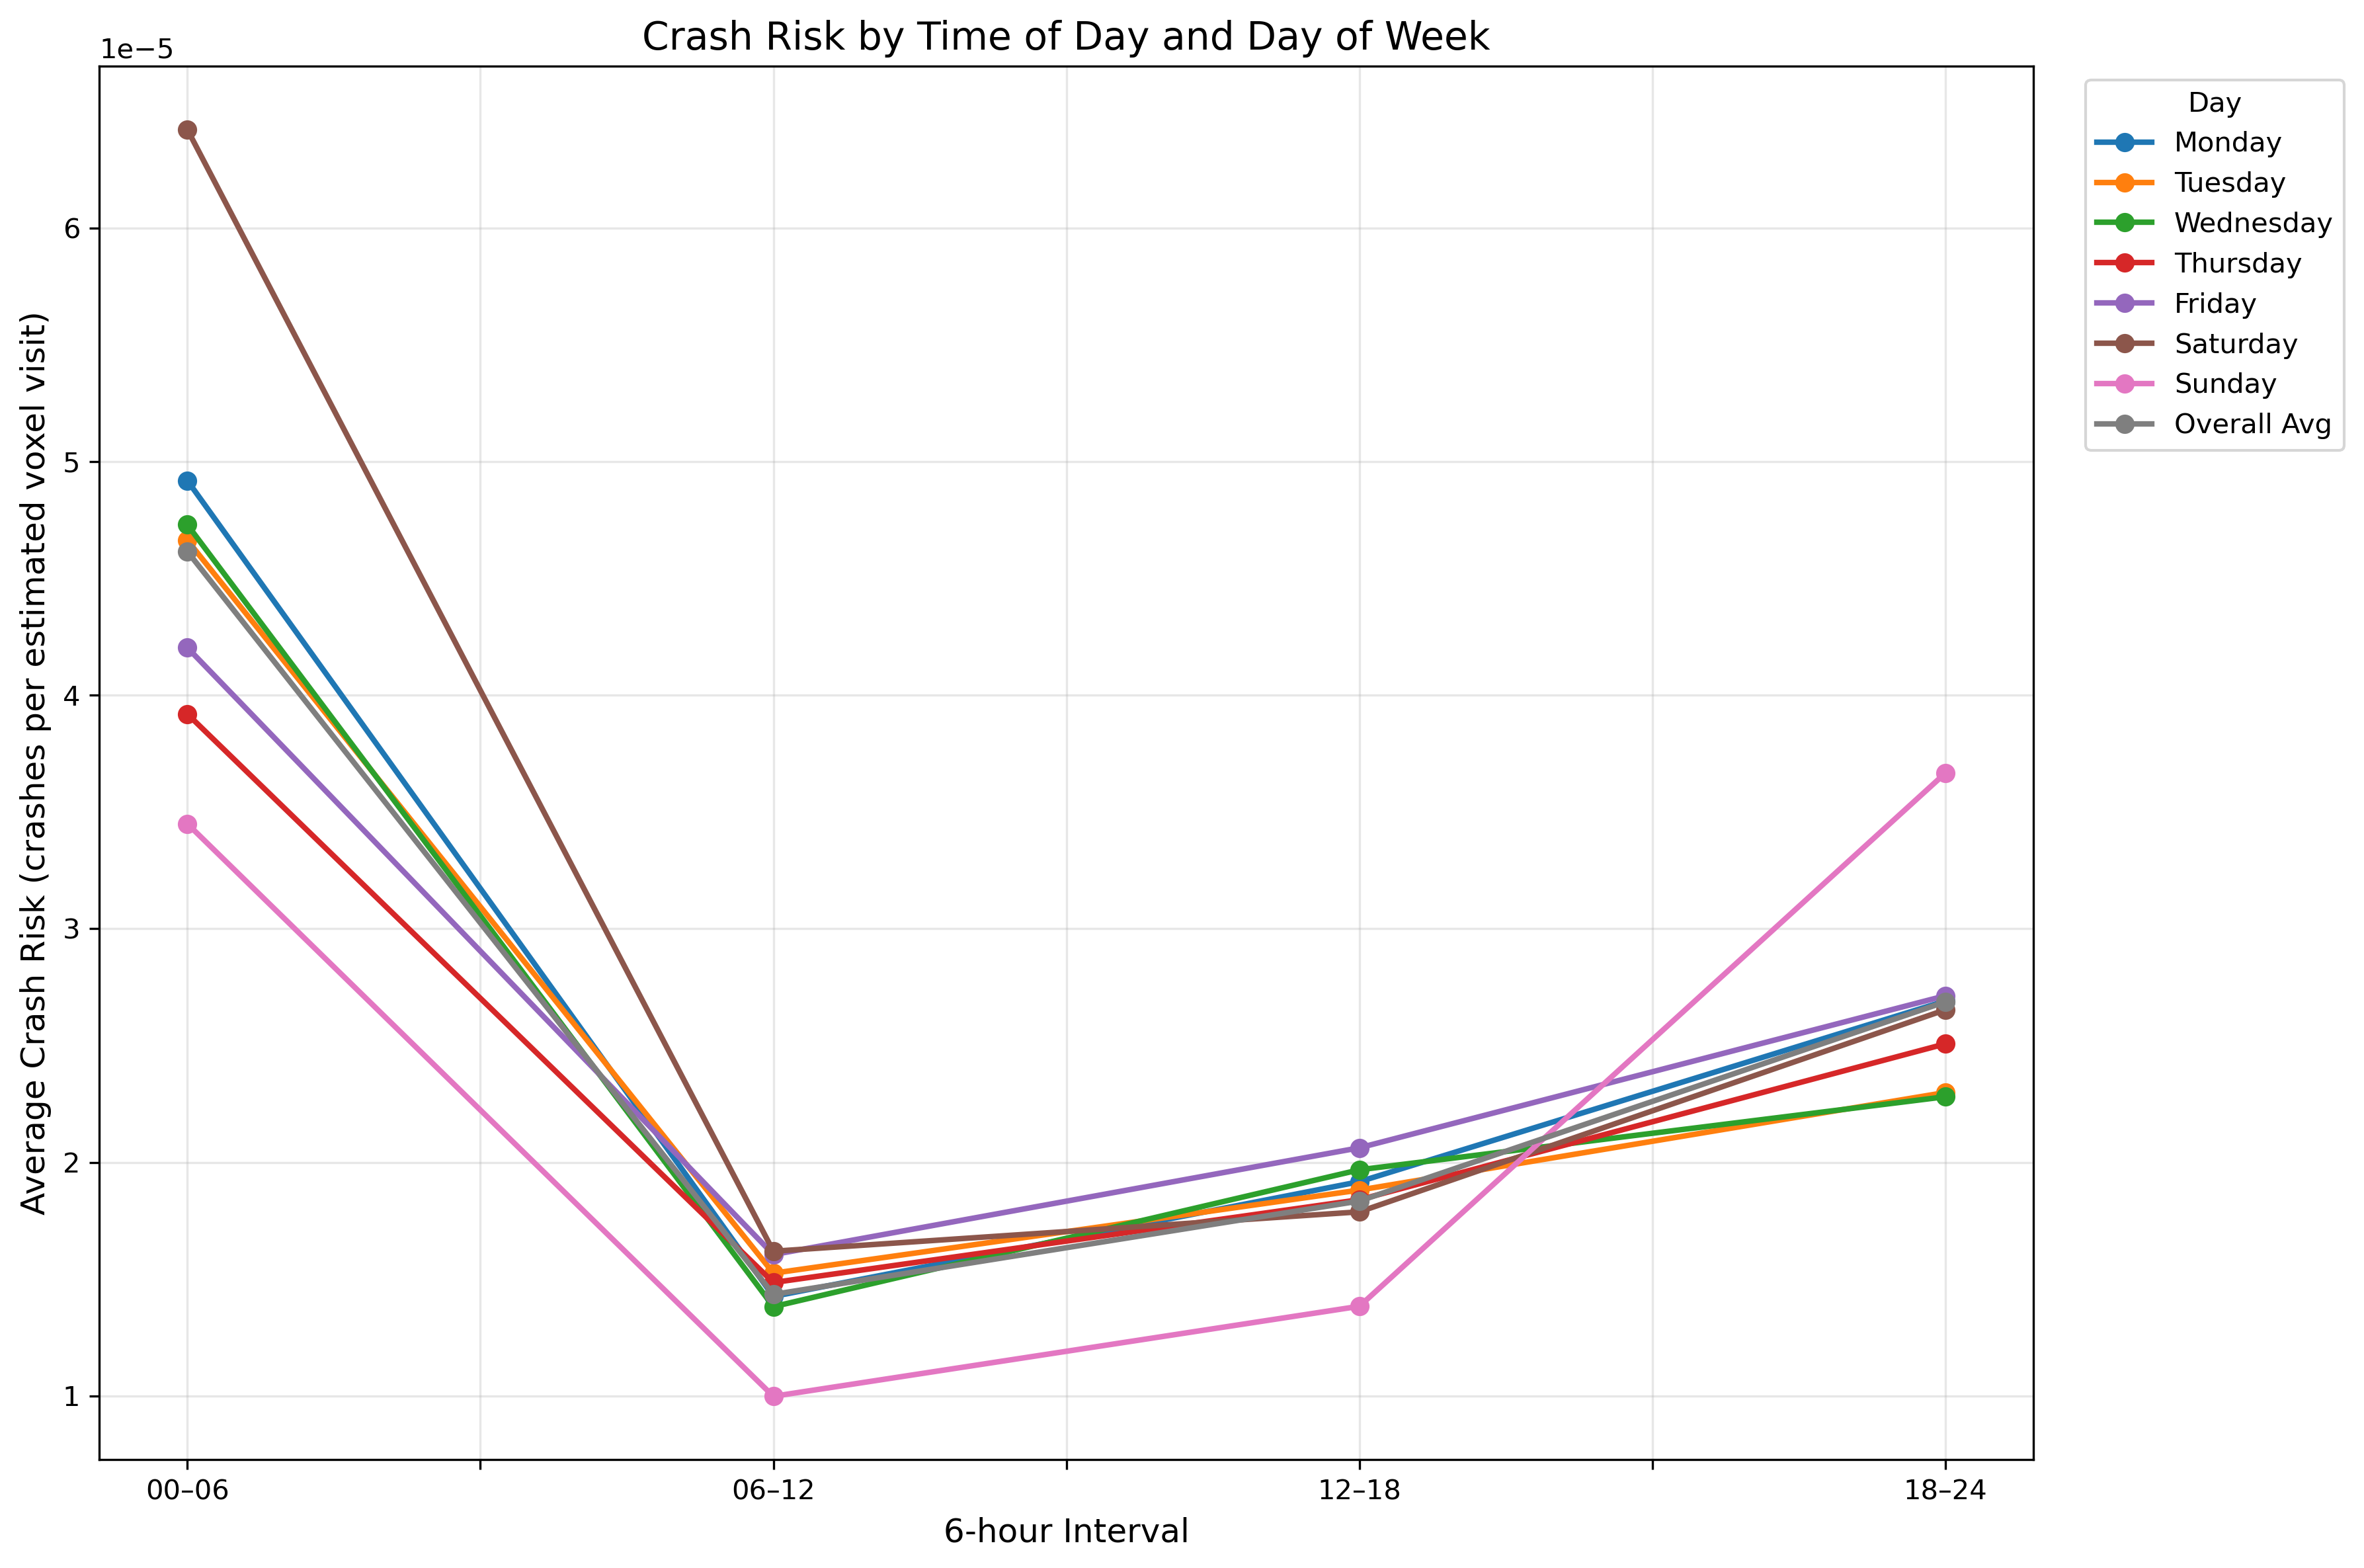
\includegraphics[width=0.9\textwidth]{../results/cellx800m_celly800m_cellt6h/plots/crash_risk_by_day_and_time_800.0m_800.0m_6.0h.png}
                \caption{Risiko variiert nach Tag und Zeit}
            \end{figure}
        \end{column}
        
        \begin{column}{0.43\textwidth}
            \begin{figure}
                \centering
                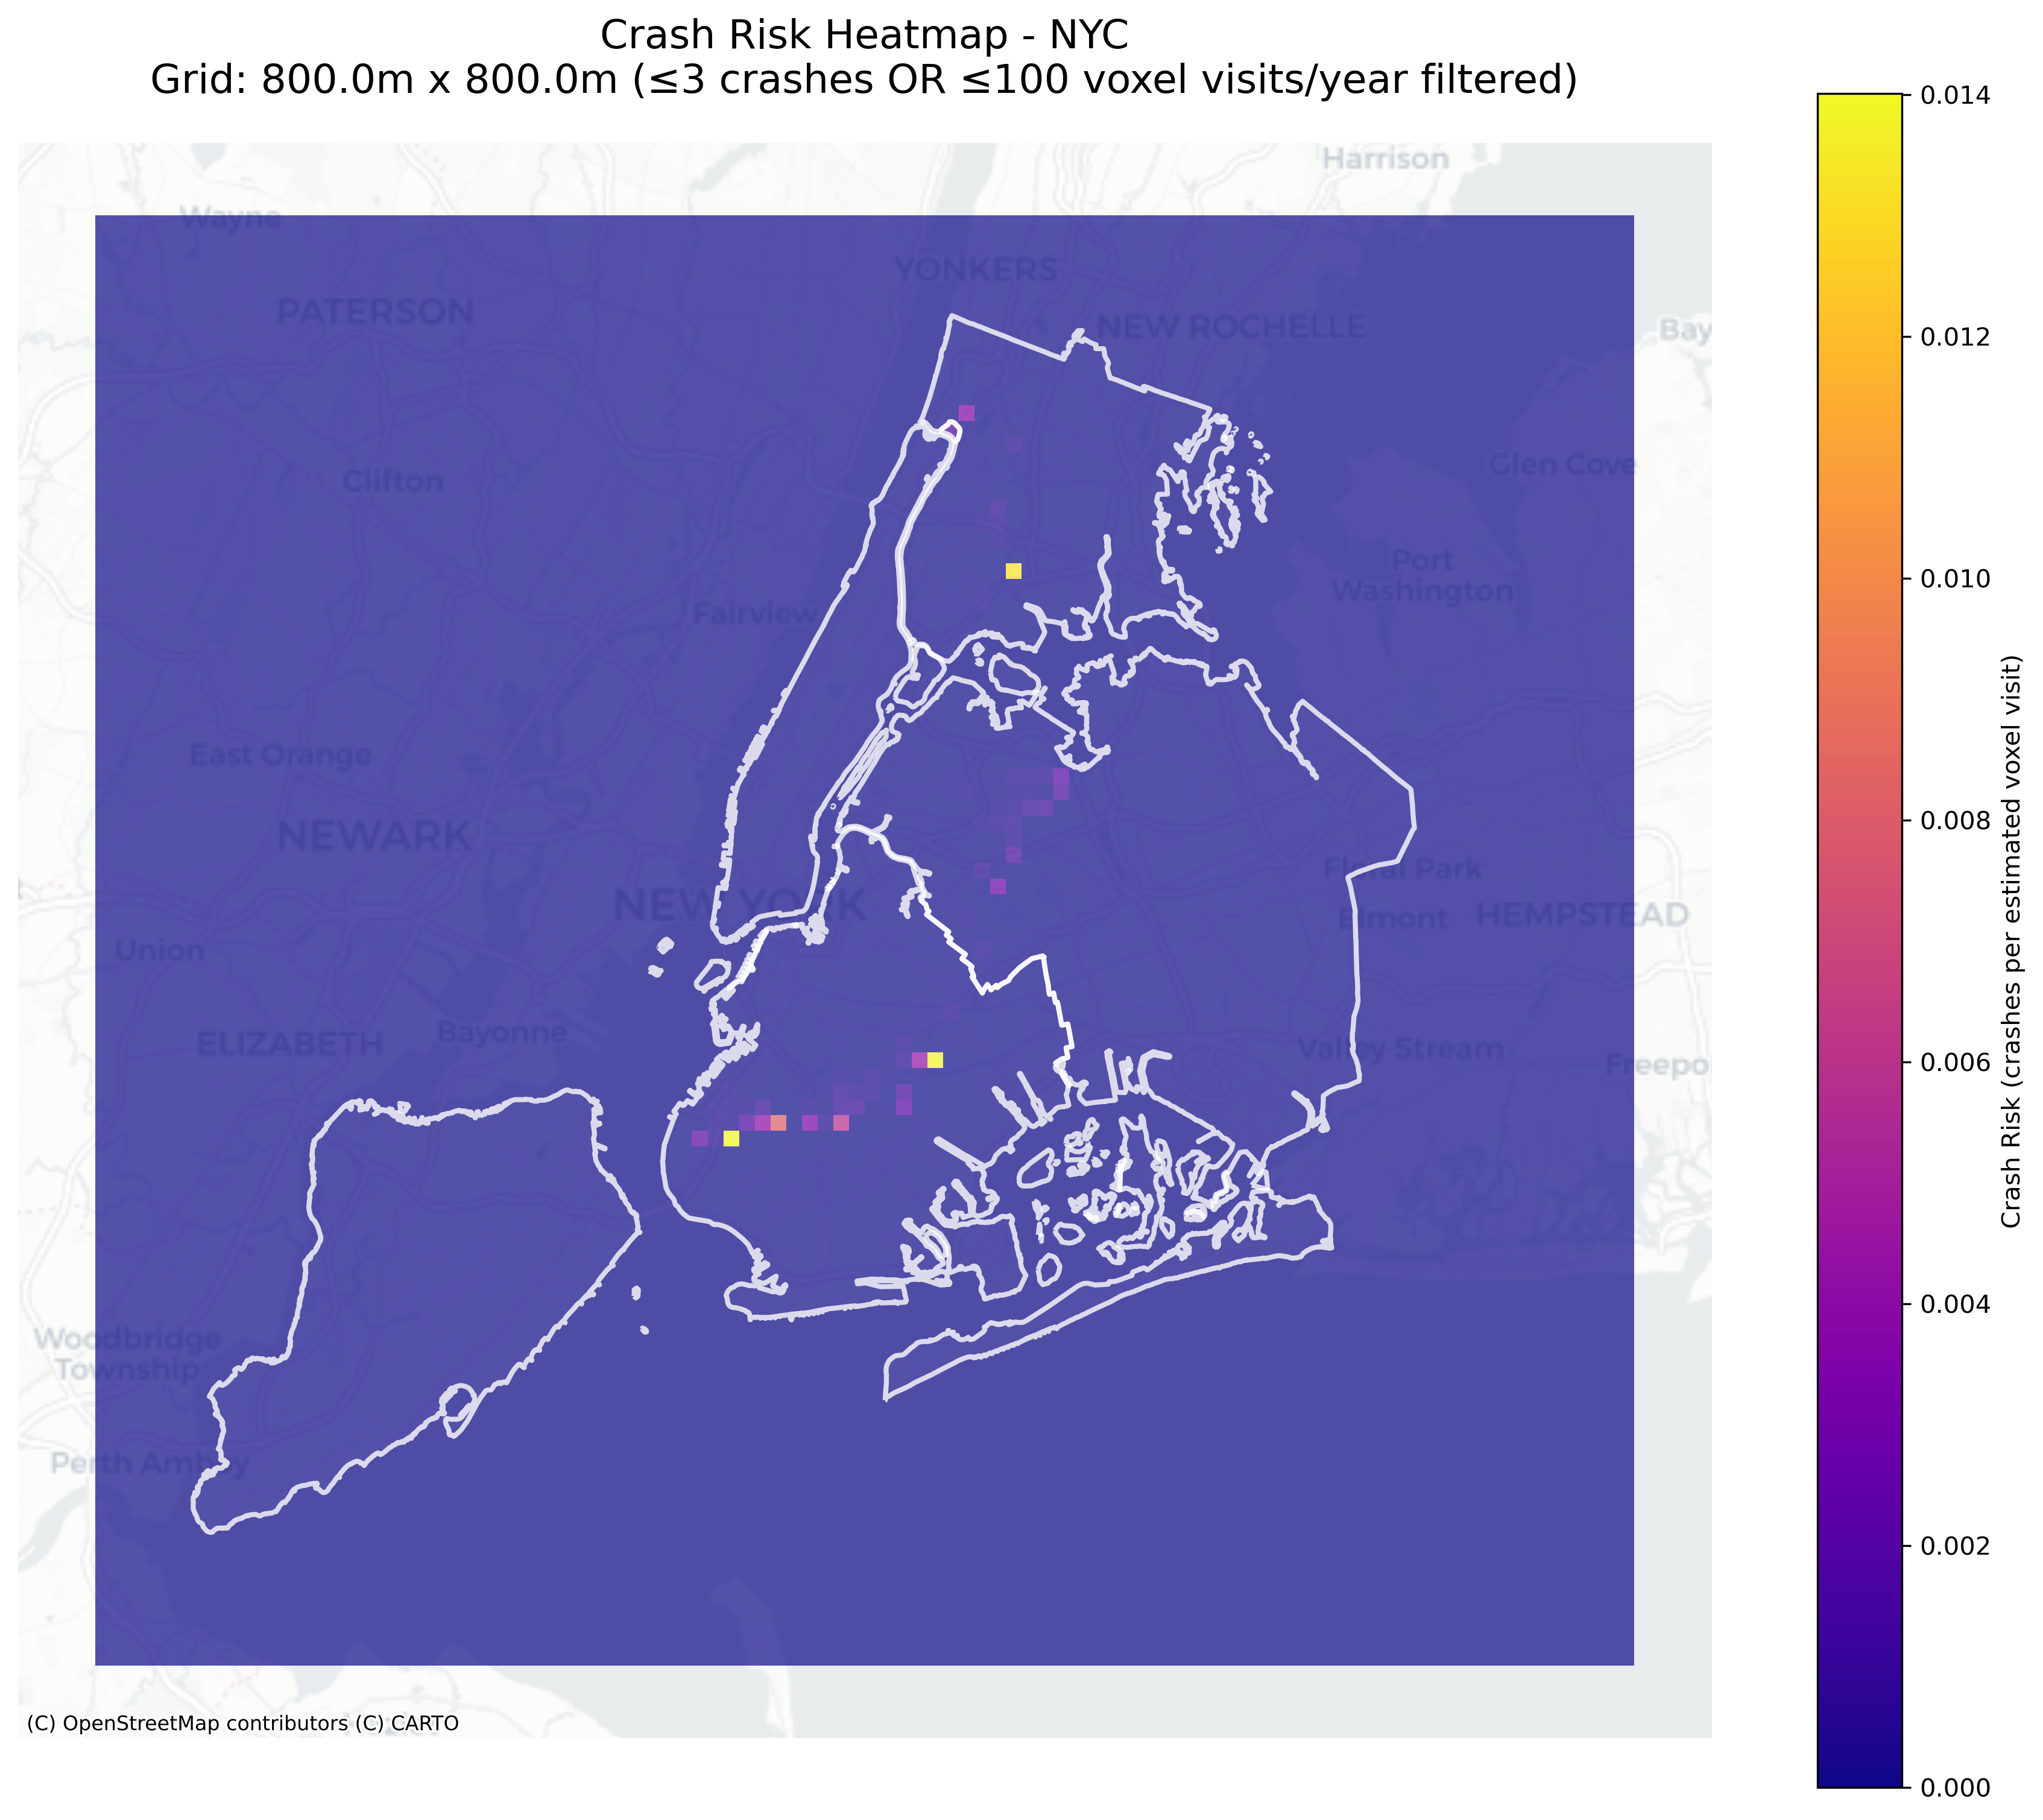
\includegraphics[width=0.9\textwidth]{../results/cellx800m_celly800m_cellt6h/plots/spatial_risk_heatmap_800.0m_800.0m_6.0h_filtered.png}
                \caption{Risiko variiert nach Standort}
            \end{figure}
        \end{column}
    \end{columns}
    
    \vspace{0.3cm}
    \centering{\textbf{Hohe räumliche und zeitliche Variabilität im Unfallrisiko}}
\end{frame}

%%%%%%%%%%%%%%%%%%%%%%%%%%%%%%%%%%%%%%%%%%%%%%%%%%%%%%%%%%%%%%%%%%%%%%%%%%%%%%%%
% Folie 5: Wechselwirkungen und Modell-Herausforderungen
%%%%%%%%%%%%%%%%%%%%%%%%%%%%%%%%%%%%%%%%%%%%%%%%%%%%%%%%%%%%%%%%%%%%%%%%%%%%%%%%

\begin{frame}{Komplexe Wechselwirkungen}
    \vspace{0.2cm}
    \begin{columns}
        \begin{column}{0.6\textwidth}
            \begin{figure}
                \centering
                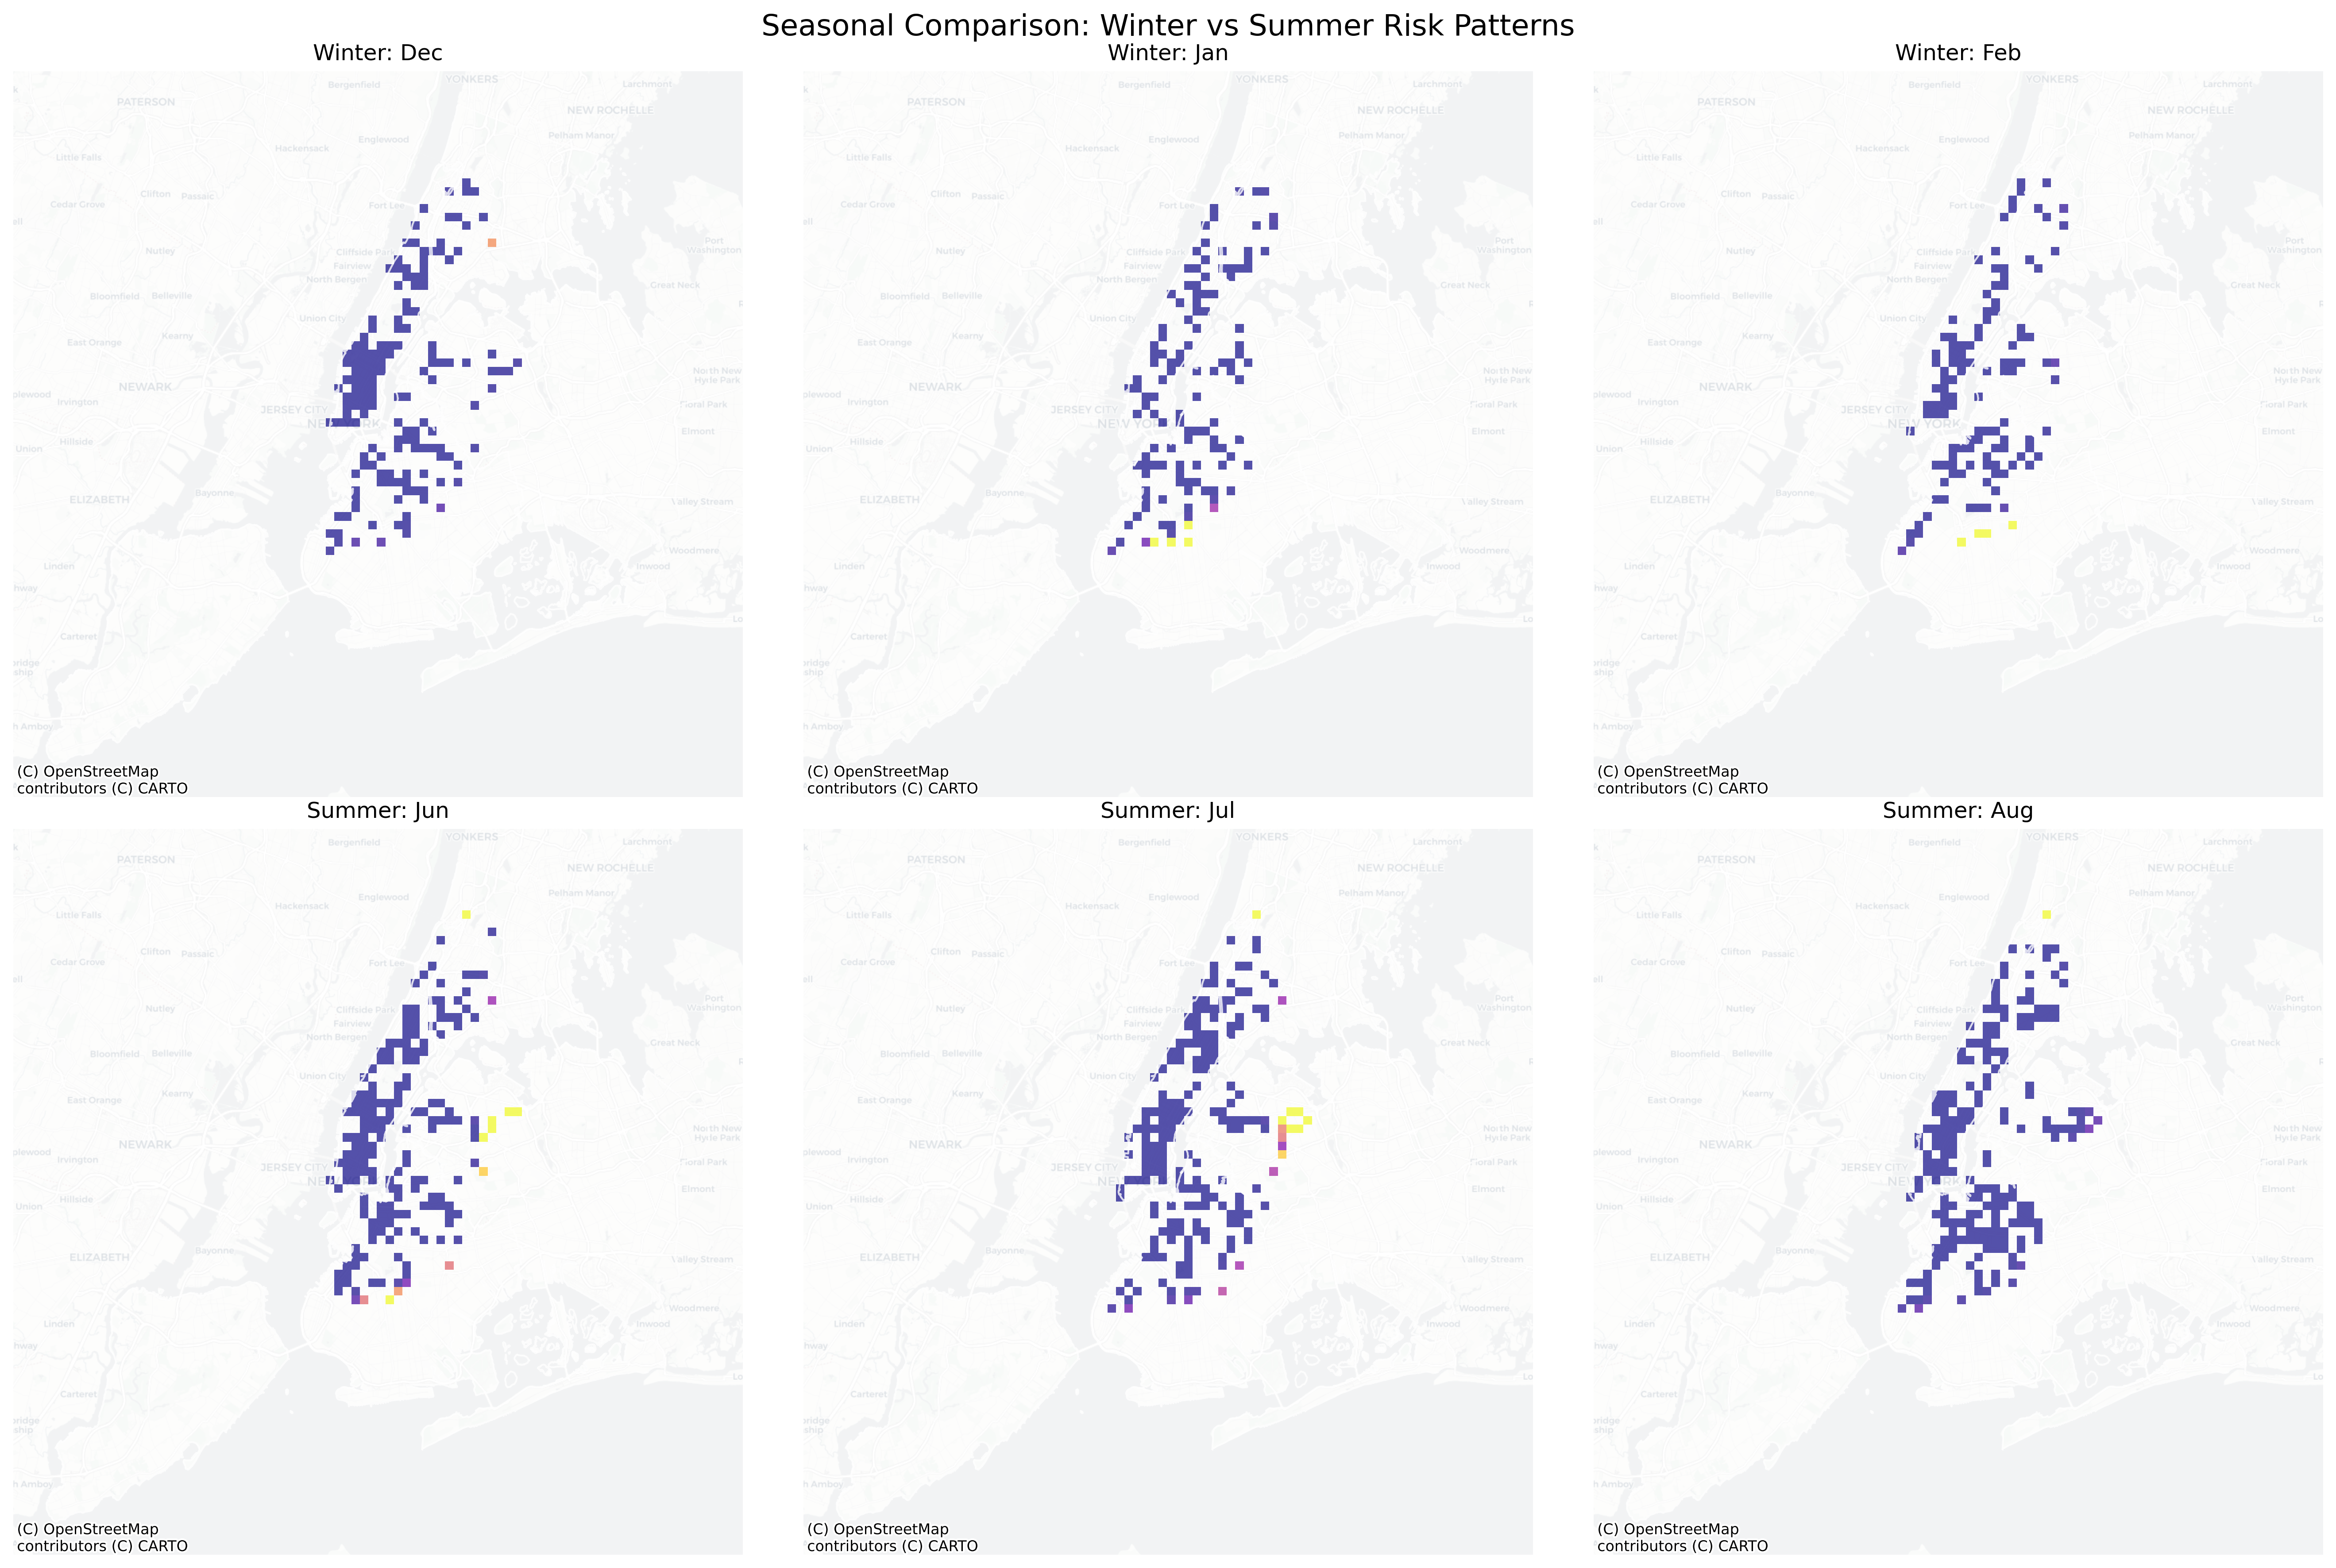
\includegraphics[width=\textwidth]{../results/cellx800m_celly800m_cellt6h/plots/seasonal_risk_comparison_800.0m_800.0m_6.0h.png}
                \caption{Saisonale Risikomuster unterscheiden sich räumlich}
            \end{figure}
        \end{column}

        \begin{column}{0.4\textwidth}
            \textbf{Problem:} Trotz grober Rasterung \\
            - räumliche Cluster sind nicht homogen und inkonsistent über Zeit \textbf{und} \\
            - Unfallfälle pro Voxel nähern sich dem Ausreißerbereich.
        \end{column}
    \end{columns}
\end{frame}

%%%%%%%%%%%%%%%%%%%%%%%%%%%%%%%%%%%%%%%%%%%%%%%%%%%%%%%%%%%%%%%%%%%%%%%%%%%%%%%%
% Folie 6: Aktuelle beste Lösung
%%%%%%%%%%%%%%%%%%%%%%%%%%%%%%%%%%%%%%%%%%%%%%%%%%%%%%%%%%%%%%%%%%%%%%%%%%%%%%%%
\begin{frame}{Aktuelle beste Lösung: Einfache, verständliche Regeln}
    \vspace{0.3cm}
    \textbf{Ehrliche Einschätzung:} Mit den aktuellen Daten allein können wir spezifische Gefahrenzonen nicht zuverlässig identifizieren. Stattdessen sollten wir uns auf einfache Regeln konzentrieren.\\
    \vspace{0.3cm}
    \begin{itemize}
        \item \textbf{Zeit-basierte Warnungen:}
        \begin{itemize}
            \item Besondere Vorsicht während Nachtstunden und Wochenenden
            \item Spitzenrisikozeiten: Freitag-Sonntag Abende
        \end{itemize}
        
        \item \textbf{Standort-basierte Leitlinien:}
        \begin{itemize}
            \item Vorsicht in Gebieten mit geringem Fahrradverkehr
            \item Erhöhte Wachsamkeit in der Nähe von Autobahnen und großen Kreuzungen
            \item Isolierte Routen während schwacher Verkehrszeiten vermeiden
        \end{itemize}
    \end{itemize}
    
    \vspace{0.4cm}
    \textbf{Zukunftsrichtung:} Gefährliche Gebiete im Voraus vorhersagen durch Integration zusätzlicher Datenquellen (Wetter, Verkehr, Ereignisse) und sorgfältige Neuanalyse durchführen.
\end{frame}


%%%%%%%%%%%%%%%%%%%%%%%%%%%%%%%%%%%%%%%%%%%%%%%%%%%%%%%%%%%%%%%%%%%%%%%%%%%%%%%%
% Folie 7: Methoden
%%%%%%%%%%%%%%%%%%%%%%%%%%%%%%%%%%%%%%%%%%%%%%%%%%%%%%%%%%%%%%%%%%%%%%%%%%%%%%%%
\begin{frame}{Implementierungsdetails}
    Für vollständige Details zur Datenverarbeitung und Analysemethoden konsultieren Sie bitte den dokumentierten Quellcode:
    \begin{itemize}
        \item \texttt{src/apps/rasterize\_data.py}
        \item \texttt{src/utils.py}
        \item \texttt{src/jupyter/vis\_results.ipynb}
    \end{itemize}
\end{frame}

\end{document}